\documentclass[a4paper,11pt]{scrartcl}

\usepackage[ngerman]{babel} 
\usepackage[T1]{fontenc}
\usepackage[utf8]{inputenc}
\usepackage{hyperref}

\usepackage{amsmath,amsfonts,amssymb}
\usepackage{graphicx}
\usepackage{siunitx}

\usepackage{epstopdf}

\setcounter{section}{8}


\begin{document}
\hfill Alexander Schnapp

\hfill Max Menges

\hfill introhpc02

\begin{center}
\underline{\Huge{Intro HPC: Blatt 8}}\\
\large{24.11.1014}\\
\end{center}


\subsection{Reading: GPU Computing}
%Voraussetzunge.
%introduction in GPU programming.
%applications.
%gpu computing in the future

\subsection{Saxpy-CUDA implementation}
In this exercise a CUDA based implemation of the saxpy workload is diskussed. Varying the problem size on the x-axis from 1KB to 10 MB
we compare the CPU computing time with the GPU computing time on the y-axis. Both axes are in logarithmic scale. One can clearly see that the GPU computing time is neglegeble expescially at high problem sizes.

\begin{figure}[htbp]
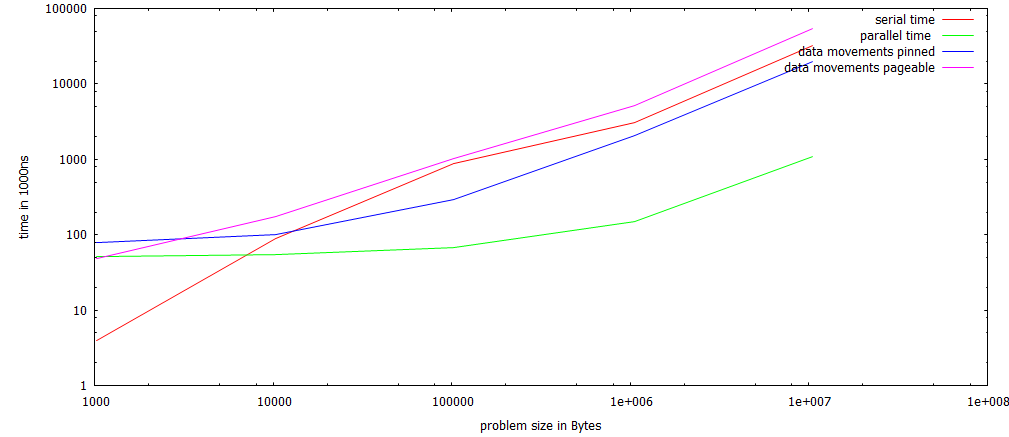
\includegraphics[width=\linewidth,
keepaspectratio]{vergleich}
\centering
\end{figure}

But you have to take care that for the GPU case you also have to consider the time of the datamovements from host to device and backwords. If you do so you see that the GPU is only in the case of a pinned memory and only except very small problem sizes faster than calculating on the CPU. 
\end{document}
